\documentclass[a4paper, 10pt]{article}
\usepackage[margin=1in]{geometry}
\usepackage[OT1]{fontenc}
\usepackage{cmbright}
\usepackage{authblk}
\usepackage{amsmath}
\usepackage{siunitx}
\sisetup{per-mode = power}
\sisetup{separate-uncertainty=true}
\usepackage{booktabs}
\usepackage{float}
\usepackage{enumitem}
\usepackage{biblatex}
\addbibresource{3b6_lab.bib}
\usepackage[hidelinks]{hyperref}
\usepackage{multicol}
\usepackage{graphicx}
\usepackage[labelfont=bf, textfont=normalfont, justification=raggedright, singlelinecheck=false, font=small]{caption}
\usepackage{pgf}
\providecommand{\mathdefault}[1]{#1} % Fix for https://github.com/matplotlib/matplotlib/issues/27907
\newcommand{\scriptfigure}[2]{
\begin{figure}
  \centering
  \input{figures/#1.pgf}
  \caption{#2}
  \label{fig:#1}
\end{figure}
}
\usepackage{titlesec}
\titleformat{\section}
  {\normalfont\bfseries}
  {\thesection}{1em}{} 
\titlespacing*{\section}{0pt}{1.2\baselineskip}{0.6\baselineskip}
\titleformat{\subsection}
  {\normalfont\itshape}
  {\thesubsection}{1em}{} 
\titlespacing*{\subsection}{0pt}{1\baselineskip}{0.4\baselineskip}

\title{Module Report\\[0.5em]
\Large 3B6 \textit{Photonic Technology}}
\author[1]{Tahmid Azam}
\affil[1]{Emmanuel College, University of Cambridge}
\date{March 2026}

\begin{document}
\maketitle

\begin{abstract}
    Semiconductor lasers are critical components in applications ranging from optical data storage to long-haul telecommunications. This experiment investigates two such devices: a CD laser operating near \SI{780}{\nano\metre} and a telecommunications laser operating near \SI{1.55}{\micro\metre}. For the CD laser, the light--current and voltage--current characteristics are measured, from which the threshold current, series resistance, and emission wavelength are extracted. For the telecommunications laser, the output spectrum is measured above and below threshold to observe the transition from spontaneous to stimulated emission, and the longitudinal mode spacing is used to calculate the effective refractive index of the waveguide.
\end{abstract}

\section{CD laser}

The driver output amplitude was set to minimum, with a pulse length of $\SI{5}{\micro\second}$
and duty cycle of $1\%$. Measuring the voltage across the $\SI{20}{\ohm}$ sense resistor at this condition gave
$V_R = \SI{55}{\milli\volt}$, corresponding to a current of $I = \frac{V_R}{R} = \frac{0.055}{20} = \SI{2.75}{\milli\ampere}$.
This confirms that current is not zero.
The laser diode begins conducting as soon as it is forward biased beyond its
turn-on voltage, consistent with standard diode behaviour.
At \SI{2.75}{\milli\ampere} this current is well below the lasing threshold of $40$--$\SI{55}{\milli\ampere}$, and no optical output is expected or observed.

The optical output and laser voltage were recorded for driving currents from 0 to $I_\mathrm{max} = I_\mathrm{th} + \qty{20}{\milli\ampere}$. The true laser voltage was obtained by subtracting the voltage drop across the \SI{20}{\ohm} monitor resistor:
\begin{equation*}
    V_\mathrm{laser} = V_\mathrm{monitor} - I \times \SI{20}{\ohm} = V_\mathrm{monitor} - V_R
\end{equation*}

\begin{table}[h]
    \centering
    \begin{tabular}{ccc}
        \toprule
        current monitor (V) & voltage monitor (V) & photodiode output (mV) \\
        \midrule
        0.987               & 2.570               & 0.000                  \\
        1.044               & 2.640               & 11.900                 \\
        1.056               & 2.655               & 15.650                 \\
        1.087               & 2.695               & 25.000                 \\
        1.131               & 2.755               & 31.900                 \\
        1.187               & 2.810               & 50.150                 \\
        1.231               & 2.865               & 57.125                 \\
        1.256               & 2.890               & 65.275                 \\
        1.288               & 2.935               & 78.800                 \\
        1.350               & 3.000               & 79.350                 \\
        1.463               & 3.135               & 101.300                \\
        \bottomrule
    \end{tabular}
    \caption{Raw measurements from investigating L--I and V--I relationships for the CD laser.}
    \label{tab:cd-data}
\end{table}

\scriptfigure{cd}{L--I and V--I plots for the CD laser.}

The threshold current is identified as the point at which the optical output begins to rise sharply by observation and from the later L--I curve:
\begin{equation*}
    I_\mathrm{th} = \qty{53.1}{\milli\ampere}
\end{equation*}
This is in line with the handout's stated range of \SIrange{40}{55}{\milli\ampere}. Considerable noise in the optical output at the oscilloscope formed a wide band, in which human estimation was used to find the midpoint and measure a value; resulting in large inaccuracies. Below threshold the device operates as an LED and spontaneous emission dominates; above threshold stimulated emission dominates.

\subsection{Finding the series resistance}

A linear regression (using \texttt{scipy.stats.linregress} in Python) of $V_\mathrm{laser}$ against $I$ for all above-threshold data points gives a slope of:
\begin{equation*}
    R_s = \SI{3.5}{\ohm}
\end{equation*}
This is the value of the series resistance. The uncertainty of regression can be calculated using the standard error of the estimated slope, assuming residual normality \cite{LinregressSciPyV1170}, and is found to be \SI{0.2}{\ohm}. The uncertainty of the individual oscilloscope measurements is captured by this quantity. However, the manufacturer tolerance of the \SI{20}{\ohm} resistor is not, which is a systematic error. The manufacturer tolerance of the \SI{20}{\ohm} resistor was not recorded; a conservative estimate of \SI{10}{\percent} is assumed, corresponding to a silver-band tolerance resistor \cite{iec60062}. Since $I = V_R / R$, a fractional error in $R$ scales all current values and hence the slope by the same fraction: $\delta R_s^{(\mathrm{sys})} = 0.10 \times 3.5 = \SI{0.4}{\ohm}$. Following Appendix B, systematic and random errors are added linearly as a conservative estimate:
\begin{equation*}
    R_s = 3.5 \pm (0.2 + 0.4) = \SI{3.5 +- 0.6}{\ohm}
\end{equation*}
The $R^2=0.962$ is indicative of a reasonably good fit and that the variance is well-described by a line.

\subsection{Finding the ideal-diode voltage $V_0$}

The intercept of this fit at $I=I_\mathrm{th}$ gives the ideal-diode voltage:
\begin{equation*}
    V_0 = \SI{1.418 +- 0.013}{\volt}
\end{equation*}
This value should not change when the laser is driven further above threshold. Above the lasing threshold, the carrier density in the active region clamps at its threshold value: additional injected current is converted into stimulated photon emission rather than increasing the carrier population. Since $V_0$ reflects the quasi-Fermi level separation, which is set by the carrier density, it remains fixed. This carrier clamping is what gives rise to the linear V--I relationship above threshold, where the only additional voltage drop is across the series resistance $R_s$.


\subsection{Finding the wavelength}

We can find the wavelength of the laser:
\begin{equation*}
    \lambda  = \frac{hc}{eV_0}
    = \frac{(6.626\times10^{-34})(3.00\times10^{8})}
    {(1.602\times10^{-19})(1.418)}
    = \SI{874.1}{\nano\metre}
\end{equation*}
This overshoots the expected 780 nm stated in the handout; the percentage error is \SI{12}{\percent}. The uncertainty in this measurement is large, errors include:
\begin{itemize}[noitemsep]
    \item the systematic error from the manufacturer tolerance in the \SI{20}{\ohm} resistor;
    \item the random error in oscilloscope measurements;
    \item the temperature effects not controlled or measured for;
    \item $V_0$ not representing the true photon energy, reflecting the quasi-Fermi level separation at threshold rather than the bandgap;
    \item the untested assumption of linearity above threshold;
\end{itemize}
The uncertainty in $\lambda = hc / eV_0$ is dominated by the uncertainty in $V_0$. Since $h$, $c$, and $e$ are known to negligible error, propagation gives $\delta\lambda / \lambda = \delta V_0 / V_0$. The regression intercept standard error gives $\delta V_0^{(\mathrm{rand})} = \SI{0.013}{\volt}$. As discussed for $R_s$, the resistor tolerance does not affect $V_0$: it scales the current axis uniformly, changing the slope but leaving the intercept unchanged. The random uncertainty in $\lambda$ is therefore:
\begin{equation*}
    \delta\lambda = \lambda \frac{\delta V_0}{V_0} = 874.1 \times \frac{0.013}{1.418} = \SI{8.0}{\nano\metre}
\end{equation*}
This ultimately gives:
\begin{equation*}
    \boxed{\lambda = \SI{874 +- 8}{\nano\metre}}
\end{equation*}
This uncertainty does not account for the systematic effects discussed above which dominate the \SI{12}{\percent} discrepancy from the expected \SI{780}{\nano\metre}.

\section{Telecommunications laser}
\subsection{Measurements}
\begin{figure}[H]
    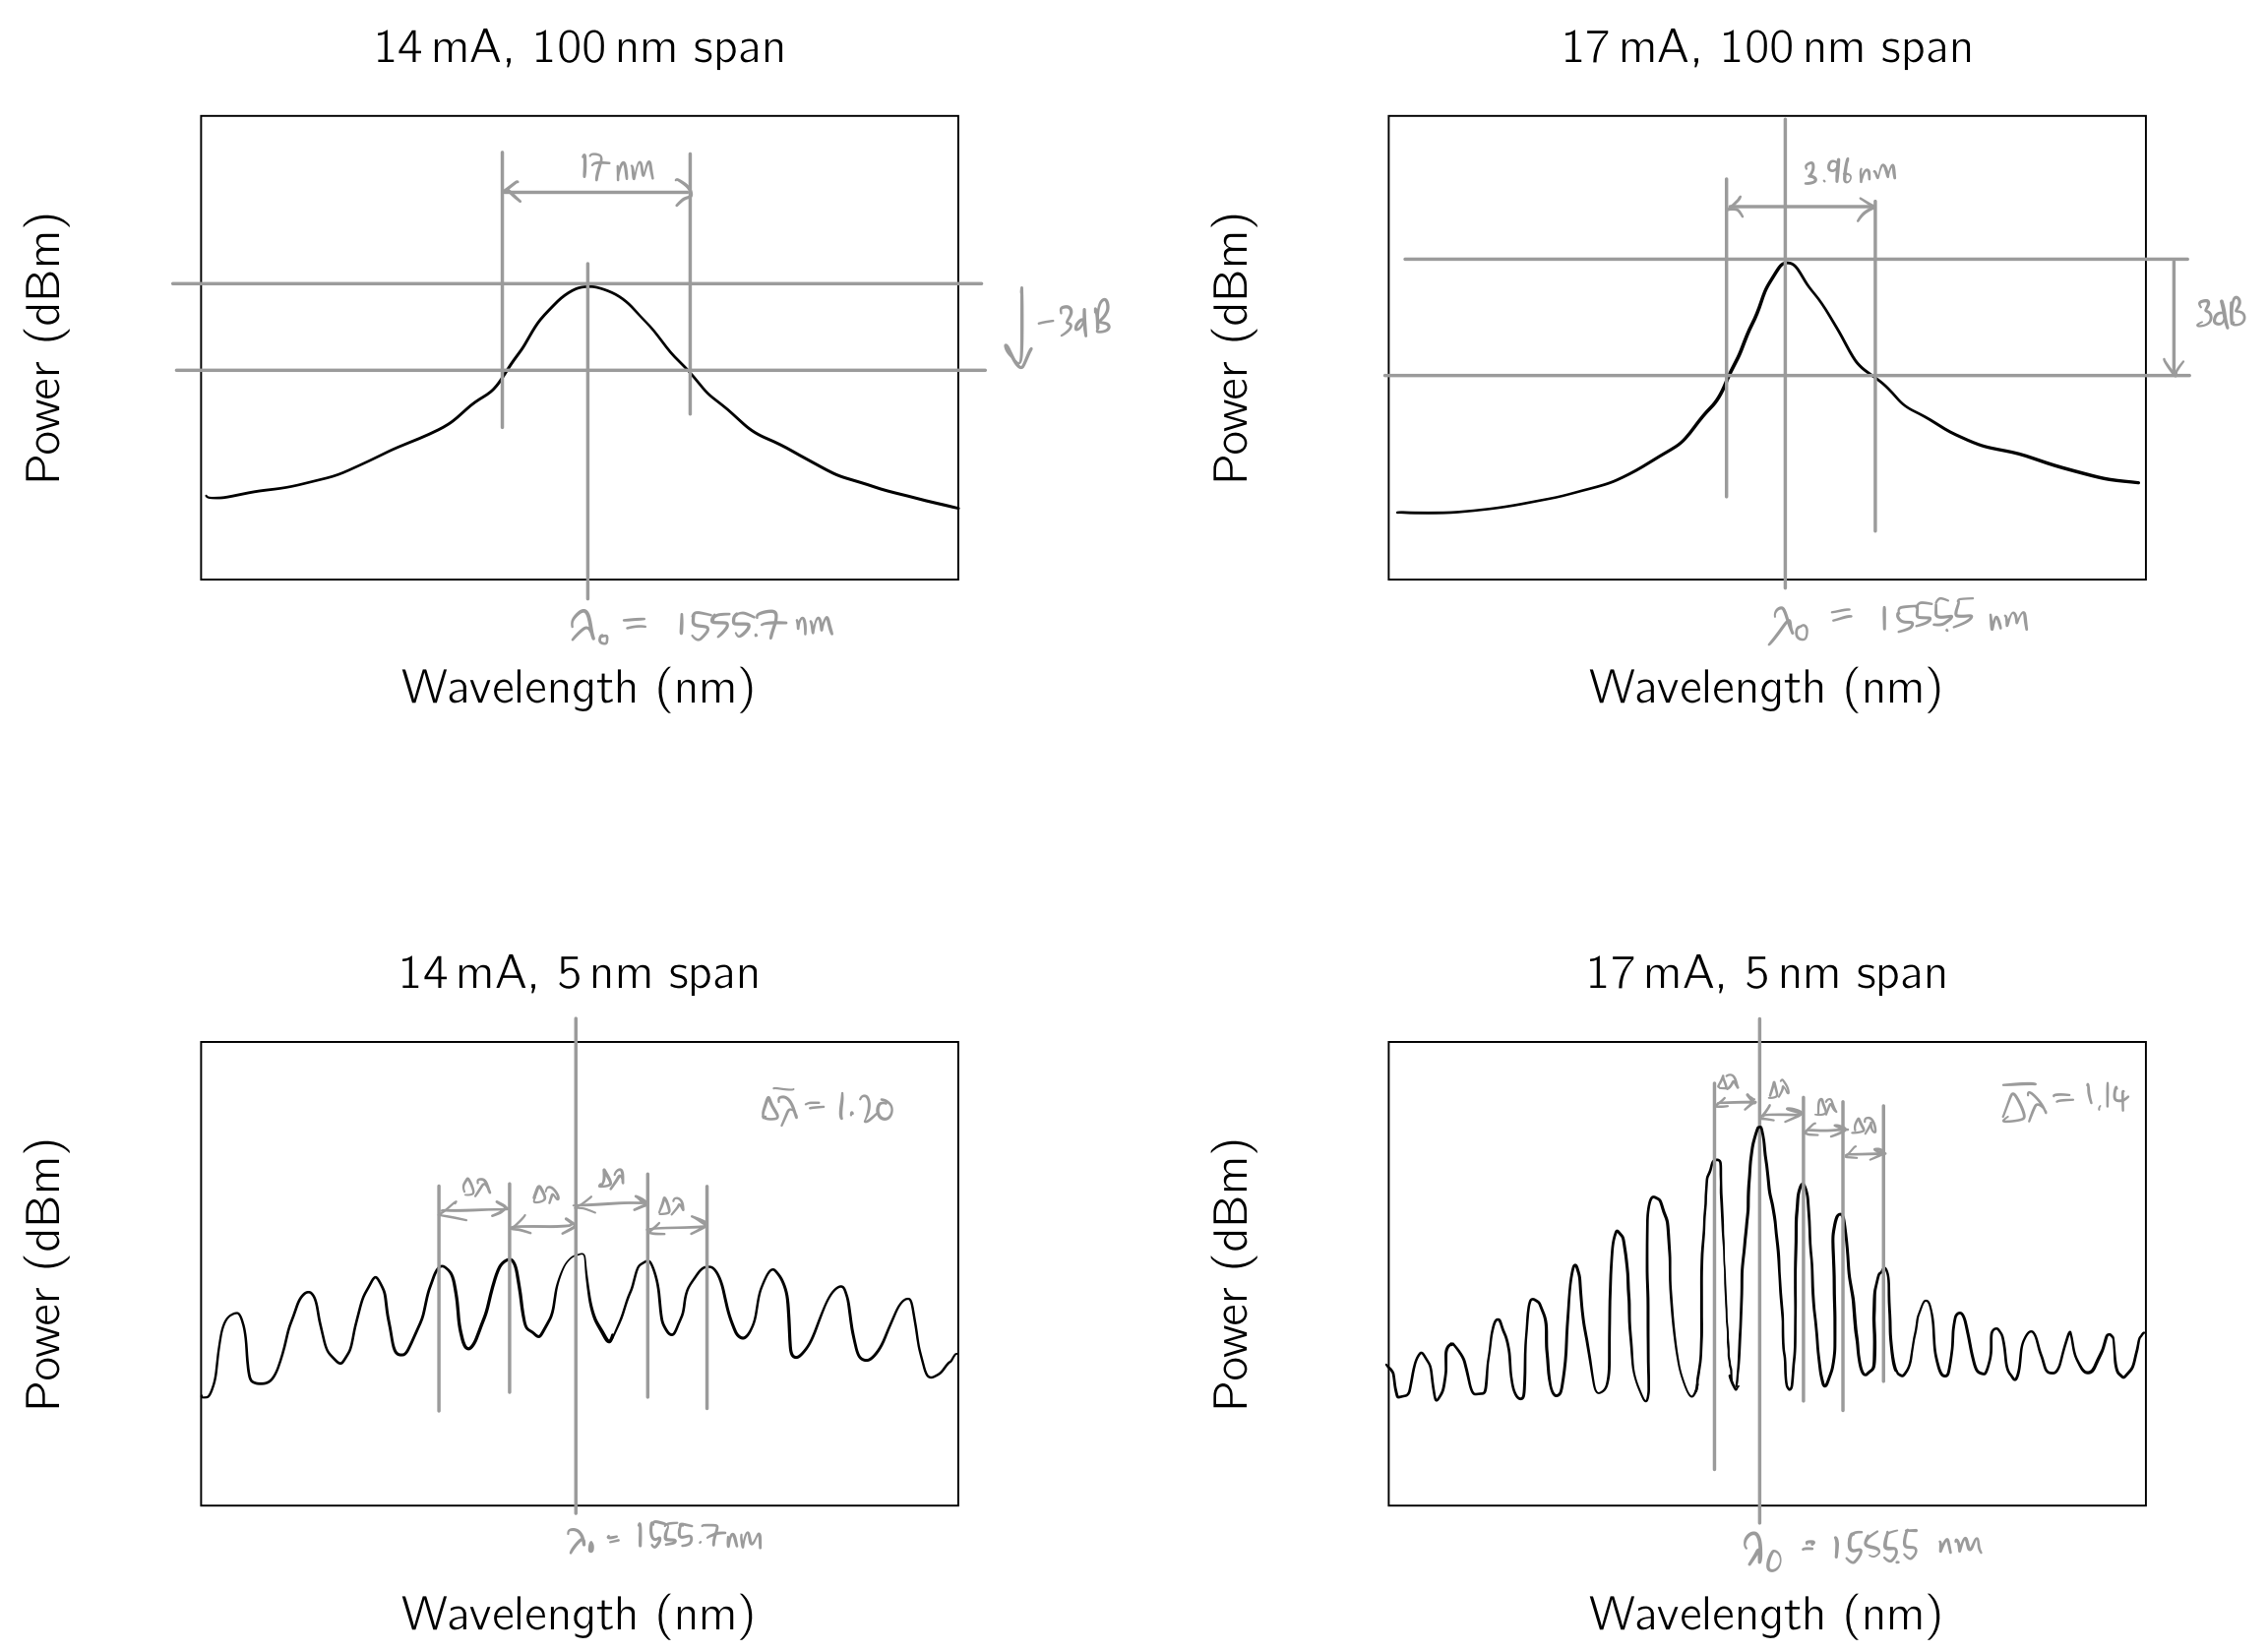
\includegraphics[width=\textwidth]{images/sketches.png}
    \caption{Sketches of the output spectrum.}
    \label{fig:sketch}
\end{figure}

\begin{table}[H]
    \small
    \centering
    \begin{tabular}{lcc}
        \toprule
                                                   & \multicolumn{2}{c}{Operating condition}                          \\
        \cmidrule(lr){2-3}
                                                   & \SI{17}{\milli\ampere}                  & \SI{14}{\milli\ampere} \\
        \midrule
        $\lambda_0$ (nm)                           & 1555.5                                  & 1555.7                 \\
        $P_0$ (dBm)                                & $-20.0$                                 & $-34.8$                \\
        3\,dB width (nm)                           & 3.96                                    & 17                     \\
        \midrule
        $\Delta\lambda_1$ (nm)                     & 1.13                                    & 1.17                   \\
        $\Delta\lambda_2$ (nm)                     & 1.15                                    & 1.22                   \\
        $\Delta\lambda_3$ (nm)                     & 1.14                                    & 1.19                   \\
        $\Delta\lambda_4$ (nm)                     & 1.12                                    & 1.24                   \\
        $\Delta\lambda_5$ (nm)                     & 1.16                                    & 1.18                   \\
        \midrule
        $\overline{\Delta\lambda} \pm \sigma$ (nm) & $1.14 \pm 0.02$                         & $1.20 \pm 0.03$        \\
        \bottomrule
    \end{tabular}
    \caption{Spectral measurements for both drive currents: centre wavelength $\lambda_0$, 3\,dB spectral width, individual mode spacing measurements $\Delta\lambda_i$, and mean mode spacing $\bar{\Delta\lambda} \pm \sigma$.}
    \label{tab:spectral_measurements}
\end{table}

\autoref{tab:spectral_measurements} summarises the spectral measurements taken at drive currents above (\SI{17}{\milli\ampere}) and below (\SI{14}{\milli\ampere}) the threshold current of \SI{15.5}{\milli\ampere}; sketches of the output spectra can be found in \autoref{fig:sketch}. Below threshold, the output spectrum is broad with a 3\,dB width of \SI{17}{\nano\metre} centred at $\lambda_0 = \SI{1555.7}{\nano\metre}$, characteristic of spontaneous emission where electrons and holes recombine across a range of energies determined by the material gain bandwidth. Above threshold, the spectrum narrows to a 3\,dB width of \SI{3.96}{\nano\metre} centred at $\lambda_0 = \SI{1555.5}{\nano\metre}$, as stimulated emission dominates: photons in the cavity modes closest to the gain peak trigger further emission of identical photons, amplifying those modes preferentially while others are suppressed. Both spectra are centred near \SI{1.556}{\micro\metre}, within the \SI{1.55}{\micro\metre} telecommunications band as expected for this laser. The peak output power increases by approximately \SI{14.8}{\deci\bel} from \SI{-34.8}{dBm} to \SI{-20.0}{dBm} across the threshold, consistent with the transition from spontaneous to stimulated emission: above threshold, the optical gain is concentrated into a few cavity modes rather than spread across the full gain bandwidth. Longitudinal cavity modes are visible in both spectra, with mean spacings of $\overline{\Delta\lambda} = \SI{1.14 +- 0.02}{\nano\metre}$ above threshold and $\overline{\Delta\lambda} = \SI{1.20 +- 0.03}{\nano\metre}$ below. Since the mode spacing is determined by the cavity geometry through $\Delta\lambda = \lambda_0^2 / 2nL$, it should be independent of drive current; the two values are broadly consistent, and the above-threshold measurement is used for subsequent calculations.

\subsection{Calculation of effective refractive index}

Using the above-threshold values with cavity length $L=\SI{300}{\micro \metre}$ we can calculate the refractive index $n$:
\begin{equation*}
    n = \frac{\lambda_0^2}{2L\Delta\lambda} = \frac{(1555.5 \times 10^{-9})^2}{2 \times 300 \times 10^{-6} \times 1.14 \times 10^{-9}} = 3.54 \text{ to 3 s.f.}
\end{equation*}
The uncertainty in the measurements here involve:
\begin{itemize}[noitemsep]
    \item $\delta\lambda_0 = \SI{0.1}{\nano\metre}$ from the last digit;
    \item $\delta L \approx \SI{1}{\micro\metre}$ from the last digit; and
    \item $\delta\Delta\lambda = \sigma / \sqrt{N} = 0.02 / \sqrt{5} = \SI{0.009}{\nano\metre}$, the standard error of the mean from our five measurements.
\end{itemize}
We use the standard error of the mean rather than the standard deviation since our result depends on the mean mode spacing. The expression for the relative error can then be evaluated:
\begin{equation*}
    \frac{\delta n}{n} = \sqrt{\left(\frac{2\,\delta\lambda_0}{\lambda_0}\right)^2 + \left(\frac{\delta L}{L}\right)^2 + \left(\frac{\delta\Delta\lambda}{\Delta\lambda}\right)^2} = \sqrt{\left(\frac{2 \times 0.1}{1555.5}\right)^2 + \left(\frac{1}{300}\right)^2 + \left(\frac{0.009}{1.14}\right)^2} = 0.009
\end{equation*}
Therefore $\delta n = 0.009 \times 3.54 = 0.03 \text{ to 1 s.f.}$, giving:
\begin{equation*}
    \boxed{n = 3.54 \pm 0.03}
\end{equation*}
This is the \textit{effective} refractive index of the waveguide mode, rather than the bulk refractive index of the active material. The optical mode extends partially into the surrounding InP cladding, which has a lower refractive index, so the effective index lies between those of the core and cladding layers. Our value of $n = 3.54$ is consistent with typical values for InGaAsP/InP waveguides at \SI{1.55}{\micro\metre}, which range from approximately 3.2 to 3.6 depending on the active layer thickness, the composition ratios $x$ and $y$ in Ga$_{1-x}$In$_x$As$_{1-y}$P$_y$ \cite{brobergRefractiveIndexIn1xGaxAsyP1y1984, bernardMidinfraredOpticalCharacterization2018}, and operating conditions such as carrier density and temperature. As noted in the handout, these composition ratios must be carefully controlled to maintain lattice matching with the InP substrate.

\subsection{Temperature effects}
The laboratory temperature was not recorded or controlled during the experiment, which is a notable omission. Temperature affects semiconductor lasers in several ways: the threshold current increases with temperature approximately as $I_\mathrm{th} \propto \exp(T/T_0)$, where $T_0$ is a characteristic temperature of the device. For the CD laser, any drift in laboratory temperature during the measurements would introduce scatter in the L--I data and shift the apparent threshold current and $V_0$, contributing to the \SI{12}{\percent} discrepancy between the calculated and expected wavelength. For the telecommunications laser, temperature drift between the two spectral measurements could account for some of the small differences in centre wavelength and mode spacing observed between the above- and below-threshold conditions.
\section{Conclusion}
The CD laser's threshold current of \SI{53.1}{\milli\ampere} fell within the expected range. The series resistance and ideal-diode voltage were found to be $R_s = \SI{3.5 +- 0.6}{\ohm}$ and $V_0 = \SI{1.418 +- 0.013}{\volt}$, giving an estimated wavelength of $\lambda = \SI{874 +- 8}{\nano\metre}$---\SI{12}{\percent} above the expected \SI{780}{\nano\metre}, attributed to the resistor tolerance, uncontrolled temperature, non-linearity, and $V_0$ not reflecting the complete photon energy. The telecommunications laser demonstrated the expected transition from broad spontaneous emission to narrow stimulated emission across threshold, with a \SI{14.8}{\deci\bel} increase in peak power. The effective refractive index was calculated as $n = 3.54 \pm 0.03$, consistent with literature values for InGaAsP/InP waveguides. Several improvements could yield more accurate results in future work. First, collecting more data points---particularly in the vicinity of threshold---would better constrain both the threshold current and the linear fit used to extract $R_s$ and $V_0$; time constraints during the session limited the number of measurements taken. Second, more careful alignment of the photodiode and adjustment of the slit would make use of a greater portion of the detector's dynamic range, reducing the relative impact of oscilloscope noise on the optical output readings. Third, recording the ambient temperature and stabilising the laser with a thermoelectric cooler would remove a significant uncontrolled variable that affects both the threshold current and the emission wavelength.

\section{Code availability}

\begingroup
You can find the source code for typesetting this report and generating figures at:

\quote{\href{https://github.com/tahmidazam/3b6-lab}{https://github.com/tahmidazam/3b6-lab}}
\endgroup

\begingroup
\renewcommand{\bibfont}{\footnotesize}
\printbibheading
\begin{multicols}{2}
    \printbibliography[heading=none]
\end{multicols}


\end{document}